\documentclass[11pt, a4paper]{article}

%% Packages
% colored hyperlinks
\usepackage[colorlinks=true,allcolors=blue]{hyperref}
\usepackage{float}
% Floats float too much. 
\usepackage[section]{placeins}
% Margin notes
\usepackage{marginnote}
% spaces
\usepackage{xspace}
\usepackage[round]{natbib}

%% page layout
\topmargin 0pt
\textheight 46\baselineskip
\advance\textheight by \topskip
\oddsidemargin 0.1in
\evensidemargin 0.15in
\marginparwidth 1in
\oddsidemargin 0.125in
\evensidemargin 0.125in
\marginparwidth 0.75in
\textwidth 6.125in

%% Shorthands
% Marginnote
\newcommand{\mnote}[1]
{\marginnote{\footnotesize \raggedright \texttt{#1}}}
% The package name
\newcommand{\sclero}{\textit{sclero}\xspace}
%%%
%\VignetteIndexEntry{Align sampling spots in photographs}
\title{Measure growth patterns and align sampling spots in photographs: \textit{sclero} tutorial}
\usepackage{Sweave}
\begin{document}

\author{Mikko Vihtakari}
\date{\today}
\maketitle

\tableofcontents


%%%%% Sweave options %%%%%%%%
\Sconcordance{concordance:sclero_tutorial.tex:sclero_tutorial.Rnw:%
1 35 1 1 0 10 1 1 4 15 1 1 2 4 0 1 2 71 1 1 2 4 0 1 2 2 1 1 2 1 0 1 1 3 %
0 1 2 2 1 1 2 19 0 1 2 3 1 1 2 4 0 1 2 5 1 1 2 5 0 1 2 50 1 1 3 2 0 1 1 %
4 0 1 2 5 1 1 2 89 0 1 2 2 1 1 2 1 0 1 1 3 0 1 2 50 1 1 2 1 0 1 1 3 0 1 %
2 3 1 1 2 1 0 1 1 3 0 1 2 1 1 1 2 14 0 1 2 5 1 1 2 1 0 1 1 12 0 1 2 4 1 %
1 2 5 0 1 2 8 1 1 2 1 0 1 1 12 0 1 2 2 1 1 2 4 0 1 2 5 1 1 2 1 0 1 1 4 %
0 1 2 7 1 1 2 1 0 1 2 5 0 1 2 17 1 1 2 1 0 5 1 3 0 1 2 2 1 1 2 5 0 1 2 %
21 1}

% Set graphics to textwidth
\setkeys{Gin}{width=1\textwidth}
%%%%%%%%%%%%%%

\reversemarginpar

\newpage

\section{Short introduction to the package}

The \sclero package for \href{http://www.r-project.org}{R} \citep{R2014} provides tools to measure growth patterns and align sampling spots in chronologically deposited materials. The package is primarily intended for the fields of sclerochronology, geology, and dendrochronology, but the functions can also be applied for other image measuring tasks. The package is developed to interact with \href{http://imagej.nih.gov/ij/}{ImageJ} \citep{Schneider2012}, a free-to-use public domain software for image processing and analysis. As the \sclero package is developed for open source software, it is free to use and the code is modifiable by anyone interested. If these modifications are distributed in other packages or software, references to the original source (type \texttt{citation("sclero")} in R) and author(s) of the particular function are required. If you use the package in a scientific publication, please cite the package, as it is written as a volunteer contribution. The package might contain errors and users should critically evaluate the results of any function before publishing them. Contributions, code-fixes, and bug-reports are welcome and should be committed on \href{https://github.com/MikkoVihtakari/sclero}{GitHub}. Persons contributing code to the package will be credited with an authorship (\textit{Authors} field in the \href{https://github.com/MikkoVihtakari/sclero/blob/master/DESCRIPTION}{DESCRIPTION} file).

\subsection{Installation}

The package is now uploaded to \href{https://cran.r-project.org/package=sclero}{CRAN}. If you want to use the developmental version (possibly with new features), please install it from GitHub using the \textit{devtools} package: 

\begin{Schunk}
\begin{Sinput}
 library(devtools)
 install_github("MikkoVihtakari/sclero", dependencies = TRUE)
\end{Sinput}
\end{Schunk}

\subsection{Features}

This tutorial, the functions, and the documentation might be subject to changes. Currently \sclero package contains following features: 

\begin{enumerate}
\item \nameref{sec:align}
\end{enumerate}

\clearpage
\section{Aligning sample spots with growth lines} \label{sec:align}

Materials that can be used as \href{http://en.wikipedia.org/wiki/Proxy_(climate)}{proxy records} in the fields of sclerochronology, dentrochronology and geology are deposited chronologically \citep{Masson-Delmotte2013}. Consequently, visible growth lines deposited within these records can be used as time markers to reconstruct growth patterns of the material back through time (Figure \ref{Fig:principle}, \citealp{Proctor2000,Sejr2002,Schone2005a,Ambrose2012}). In general, these materials do not grow linearly, complicating the dating of geochemical samples from proxy records \citep{Schone2008,Ambrose2012}. For example, spot samples acquired with laser-ablation inductively-coupled-plasma mass-spectrometry (LA-ICP-MS) or similar techniques along the sampled material are often measured as a distance from a defined position, such as the shell margin in bivalve mollusks, and these distances are then related to time using a variety of geochemical proxies (Figure \ref{Fig:principle}, \citealp{Vihtakari2014}). Sample spots, however, have to be consistently related to the visible growth lines prior time estimates for each sample spot can be acquired (Figure \ref{Fig:principle}). This is because material in proxy records is related to time following the growth rate of the material, and growth lines mark consistent time intervals within these records. 

\begin{figure}[h]
\begin{center}
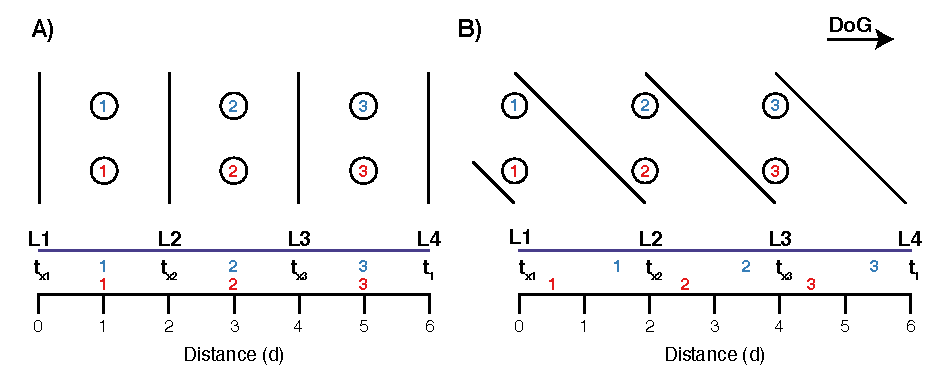
\includegraphics[width=1\textwidth]{principle.pdf}
\caption{Two sample spot sequences (blue and red numbers inside circles) taken with direction of growth (DoG) along a chronologically deposited material. Growth lines (black lines) mark consistent time intervals (t) relative to a distance from a point with a known time (d) and growth rate of the material (see text). \textbf{A)} Growth lines are vertical and both sample spot sequences are perpendicular to the growth lines. Consequently, the vertical position of sample spots does not affect the distance between sample spots and growth lines, and therefore samples taken vertically on top of each other represent the same time intervals (colored numbers without circles above the distance axis). \textbf{B)} Growth lines are at a 45$^\mathrm{o}$ angle to direction of growth, and therefore sample spot sequences are aligned in an angle to the growth lines. Consequently, the sample spots taken on top of each other do not represent the same time intervals. The \sclero package helps aligning sample spots in both examples correctly using distances from the margin along a distance axis and relative distances of sample spots from adjacent growth lines (see Figure \ref{Fig:traverse}).}
\label{Fig:principle}
\end{center}
\end{figure}

The importance of the angle between sample spot sequences and growth lines can be illustrated using two simplified examples: the first example (Figure \ref{Fig:principle}A) represents a proxy record where growth lines are at a right angle to sample spot sequences and the direction of growth, such as umbo sections of bivalve shells, tree cross-sections, otoliths, as well as sediment-, rock-, ice- or tree-cores. The three first growth lines from the left (L1, L2, and L3) are deposited after each other at unknown time intervals ($t_{x} = t_{1} - \frac{d}{\bar{r}_{x}}$, where d is the distance from L4 to the growth line of interest along the distance axis, i.e $d_{L4} - d_{Lx}$; and $\bar{r}_{x}$ is the average growth rate of the material between $d_{Lx}$ and $d_{L4}$). The last growth line on the right represents the margin or the end of the sample material often associated with a known time (t = 1 in this example). Calculating the distance of sample spots along the distance scale, which also represents a relative time scale (see the equation above), is straightforward requiring drawing a straight line from sample spots down to the axis leading to distance values of 1, 3, and 5 for both sequences. Some proxy materials, such as margin sections of bivalve shells and heavily bended sedimentary rocks do not, however, allow positioning the sample spot sequences perpendicularly to growth lines. In the second example the sample spot sequences meet growth lines at a 45$^\mathrm{o}$ angle (Figure \ref{Fig:principle}B). Now both sample spot sequences would yield distance values of 0, 2, and 4, if distance calculation was done similarly to the first example. However, this would lead to a bias when estimating time for each sample spot as the sample spots are obviously not consistently related to the growth lines. To correct for this bias, the sample spots must be related to adjacent growth lines (see Figure \ref{Fig:traverse}). This approach gives distance values of 1.5, 2.5, and 5.5 for the blue sequence and 0.5, 2.5, and 4.5 for the red sequence. These distance estimates correspond better with the chronological nature of proxy materials. The distance axis in both examples represents the historical location of the margin allowing direct growth rate calculations, if the time for each sample spot can be estimated.

The \sclero package together with ImageJ enables alignment of sample spots with visible growth bands from photographs of the sampled material. Despite the simplified example above, the \sclero package automatically calculates the location of sample spots no matter how non-linear the growth lines are as long as they do not cross at any point. In addition the package estimates the extent of sample spots along the distance axis (see Section \ref{sec:averaging_error}). This extent can be further used in estimation of time-averaging error \citep{Goodwin2004, Beelaerts2008}. In order to align the samples, the user has to define a distance axis (called `main axis' in the package) to which all sample spots and growth lines will be aligned (Figures \ref{Fig:marked} and \ref{Fig:traverse}). 

\subsection{Prerequisites for sample spot alignment}

In order to run the sample spot alignment, a photograph of sufficient resolution to see the growth lines and sample spots is required (Figure \ref{Fig:marked}). In addition, the user should take care that following points are considered:

\begin{description}
\item[Aspect ratio] The aspect ratio of pixels in the photograph has to be 1:1, meaning that a certain length vertically equals to the same length horizontally. 
\item[File format] The image file can be of any raster format compatible with ImageJ, but .tif images are generally recommended for editing purposes as this format is lossless meaning that it can be saved again without losing information. %Please note that using vector image formats (.gif, .png, .esp, .pdf) is probably not a good idea when doing measurements from photographs.
\item[Compiled images] If you are using compiled images from a microscope software, pay a special attention in aligning the photographs correctly as this will affect the results. Make sure that all compiled images are taken with a same magnification.
\item[Scaling] If you want real distances as output, the microscope has to be calibrated. If real distances are not important, knowing the microscope calibration is not essential as sample alignment is relative to one photograph. Currently there is no way to export the `Set Scale' option from ImageJ and the scaling has to be conducted using the \texttt{read.ijdata} function.
\item[Cracks] The sample material has to be chronologically deposited without spatial caps or cracks. If your sample material has large caps or cracks, they are bound to affect the output. One option is to edit the photograph in a photo editing program and remove these cracks.
\end{description}

\subsection{Mark sample spots and growth lines in ImageJ}

We use a shell margin of a bivalve shell cross-section as an example (see \citealp{d18O_paper} for details). The example file can be downloaded from \href{https://github.com/MikkoVihtakari/sclero/blob/master/inst/extdata/shellspots.png}{GitHub in .png format}. The quality of the file is not optimal due to file size restrictions, but will suffice for this example. The example shell has one sequence of samples taken with LA-ICP-MS (the large holes, Figure \ref{Fig:marked}). The work-flow can also be applied for multiple sequences of samples (see Section \ref{sec:multiple}). First we have to mark the sample spot centroids and growth lines using ImageJ. Click \href{http://imagej.nih.gov/ij/docs/guide/user-guide.pdf}{this link} for instructions how to use ImageJ. Note that, in general, all marks with ImageJ should be done \textbf{against the direction of growth}. Otherwise the aligning functions might not work properly.

\begin{figure}[H]
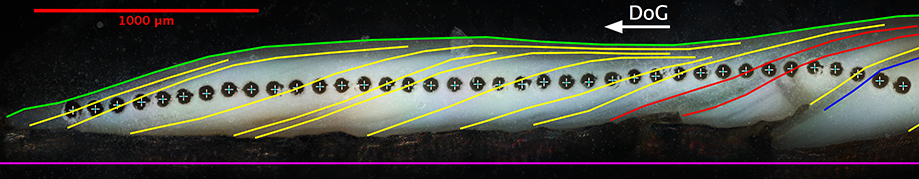
\includegraphics[width=1\textwidth]{marked_shell.pdf}
\caption{ImageJ annotated bivalve shell section. Large holes marked with crosses represent LA-ICP-MS sample spots. Colored lines on the shell section indicate the ImageJ marked growth lines, green line further representing the shell margin, yellow lines sub-annual growth lines, red lines the extent of a winter growth band, and blue line a growth line with a known time. Note that the green line (shell margin) covers the entire shell section, whereas other growth lines are long enough to align sample spots chronologically. White arrow marked `DoG' points towards the direction of growth. The magenta straight line represents the distance (main) axis. The main axis should not cross any growth line when \texttt{type} is "along". If \texttt{type} is "cross", the main axis has to cross all growth lines (see Section \ref{sec:settings}). Colors are used here only for illustration purposes and are ignored by the \sclero package.}
\label{Fig:marked}
\end{figure}

\begin{enumerate}
\item Start by using the `Multi-point Tool' and mark LA-ICP-MS sample spot centroids (see Figure \ref{Fig:marked}). The sample spots will be numbered in the order you mark the spots. In this example we begin from the margin and mark the spots against the direction of growth. The location of points marked with ImageJ is considered as the accurate location of each LA-ICP-MS spot, unless the spatial averaging-error estimation procedure is used in addition (explained in Section \ref{sec:averaging_error}).
\begin{figure}[H]
\begin{center}
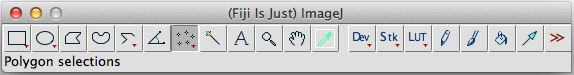
\includegraphics[width = 0.8\textwidth]{multi_point.png}
\end{center}
\end{figure}
\item After this open the ROI manager and add the sequence using Add[t] button (the keyboard shortcut is \textit{Ctrl + T} or \textit{Cmd + T} depending on the OS). You can rename the ROI (Region Of Interest) to correspond the type of the object (`Laser') for your own reference. The ROI names can be assigned as object names in consequent R functions, although this behavior is not required (see Section \ref{sec:read.ijdata}). If you decide to do this, use \texttt{\_} or \texttt{.} as a separator marker. Do not use other special characters (\texttt{-} \texttt{,} \texttt{\#}) or white space in ROI names, which you want to keep, because these will confuse the internal \texttt{grep} functions. ImageJ automatically generates ROI names containing \texttt{-} (0782-4756 for instance). These names are not valid \texttt{vector} names in R and will be regenerated by the functions in the \sclero package.
\begin{figure}[H]
\begin{center}
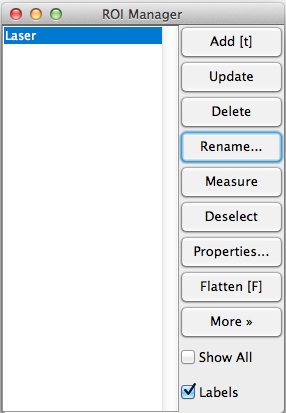
\includegraphics[width = 0.25\textwidth]{roi_manager.png}
\end{center}
\end{figure}
\item After this mark the visible growth lines using `Segmented Line' tool starting from the lower margin upwards \textit{against the direction of growth}. Mark each line so that the sample spots are in between at least two lines, but it is not necessary to continue marking much further (Figure \ref{Fig:marked}). Add each line separately to the ROI manager. The order of lines is not important as this can be changed later. Often it is easiest to start with the most clear growth lines and add less clear growth lines in between these lines as needed. Pay special attention that the \textbf{growth lines do not cross each other}. Further, there must be \textbf{at least one growth line before and after the first and last sample spot} (note the short yellow line on the right in Figure \ref{Fig:marked}). It might be helpful to rename the growth line ROIs, so that they are easier to associate later. 
\begin{figure}[H]
\begin{center}
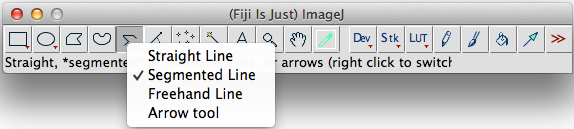
\includegraphics[width = 0.8\textwidth]{segmented_line.png}
\end{center}
\end{figure}
\item Once you are done with this, add the measurement axis using the `Straight Line' tool. It is very important to \textbf{start the axis from where you want the measurements to begin} as all distances will be scaled to this axis. The main axis should not cross any growth line, if the axis is intended to be approximately parallel to the growth lines (cores and shell sections). If your sample material is a cross-section of a tree or coral or an umbo region of a bivalve, the main axis has to cross all growth lines (see Section \ref{sec:settings}). Note that it is possible to have only one Straight Line per ImageJ .zip file as the internal functions recognize the straight line as the main axis automatically. 
\item After this you can save the ROI collection as a .zip file (More, Save...) naming it `shellspots.zip'.
\end{enumerate}

\subsection{Reading ImageJ zip files containing ROI objects} \label{sec:read.ijdata}

Next we can open R and load the \textit{sclero} package.

\begin{Schunk}
\begin{Sinput}
 library(sclero)
\end{Sinput}
\end{Schunk}

\mnote{read.ijdata} After this we use \texttt{read.ijdata} function to read and process the ImageJ .zip file containing ROIs. The code below is possible to run without having saved `shellspots.zip' file. If you followed the example above, replace `path' with the location of your ImageJ .zip file. 

\begin{Schunk}
\begin{Sinput}
 path <- file.path(system.file("extdata", package = "sclero"), "shellspots.zip")
 dat <- read.ijdata(path, scale = 0.7812, unit = "um") 
\end{Sinput}
\end{Schunk}

Note that we specified the \texttt{scale} and \texttt{unit} arguments in \texttt{read.ijdata} function, since the example photograph was calibrated. This step is not necessary, but produces actual distances instead of pixel distances ($\mathrm{\mu m}$ in this example; note that directly using $\mathrm{\mu}$ in R as a character works in some operating systems). The function returns a list of class \texttt{IJDATA} containing information about ROIs.

\begin{Schunk}
\begin{Sinput}
 summary(dat)
\end{Sinput}
\begin{Soutput}
               Length Class      Mode     
spots.x         1     data.frame list     
spots.y         1     data.frame list     
gbs.x          14     data.frame list     
gbs.y          14     data.frame list     
main.x          1     data.frame list     
main.y          1     data.frame list     
sample.name     1     -none-     character
scaling.factor  1     -none-     numeric  
unit            1     -none-     character
\end{Soutput}
\end{Schunk}

\mnote{\mbox{order}.
\mbox{ijdata}} At this point it can be of interest to reorder some of the ROIs. The order of ROIs does not make a difference in subsequent calculations, but the output will be given in the order the of IJDATA object. \texttt{order.ijdata(..., print.order = TRUE)} function can be used to check the order of ROIs.

\begin{Schunk}
\begin{Sinput}
 order.ijdata(dat, print.order = TRUE)
\end{Sinput}
\begin{Soutput}
$spots
           Laser
col.number     1

$gbs
           margin calcein l3 WG_start WG_end l6 l7 l8 l9 l10 l11 l12 l13 l14
col.number      1       2  3        4      5  6  7  8  9  10  11  12  13  14
\end{Soutput}
\end{Schunk}

The same function can be used to reorder and subset ROIs within IJDATA objects. Subsetting can be done by leaving out the elements you do not want to include in the IJDATA object. In the case of subsetting the function prints a warning to make sure that the user did not forget to specify all elements within the object. Say that we want to reorder the growth lines:

\begin{Schunk}
\begin{Sinput}
 dat2 <- order.ijdata(dat, gbs = c(1,3,6:14,4,5,2))
 order.ijdata(dat2, print.order = TRUE)
\end{Sinput}
\begin{Soutput}
$spots
           Laser
col.number     1

$gbs
           margin l3 l6 l7 l8 l9 l10 l11 l12 l13 l14 WG_start WG_end calcein
col.number      1  2  3  4  5  6   7   8   9  10  11       12     13      14
\end{Soutput}
\end{Schunk}

\mnote{\mbox{convert}.
\mbox{ijdata}} The information in IJDATA objects is meant to be user modifiable. The object behaves like any \texttt{list} in R only that the name of elements (\texttt{\$spots.x, \$spots.y, ...}) should not be changed to ensure that subsequent functions work correctly. In order to align the sample spots along the main axis, we need to convert the information to \href{http://www.spatstat.org/spatstat/}{\textit{spatstat}} \citep{Baddeley2005} objects using \texttt{convert.ijdata} function.

\begin{Schunk}
\begin{Sinput}
 shell <- convert.ijdata(dat)
\end{Sinput}
\end{Schunk}

\mnote{plot.
rawDist} The function returns a list of class \texttt{rawDist}, which can be plotted using the generic plotting function. The plot will be a representation of the ROIs, with the exception that the coordinate system is flipped vertically. This is because of coordinate system differences between Java (ImageJ) and R.

\begin{figure}[H]
\begin{center}
\begin{Schunk}
\begin{Sinput}
 plot(shell)
\end{Sinput}
\end{Schunk}
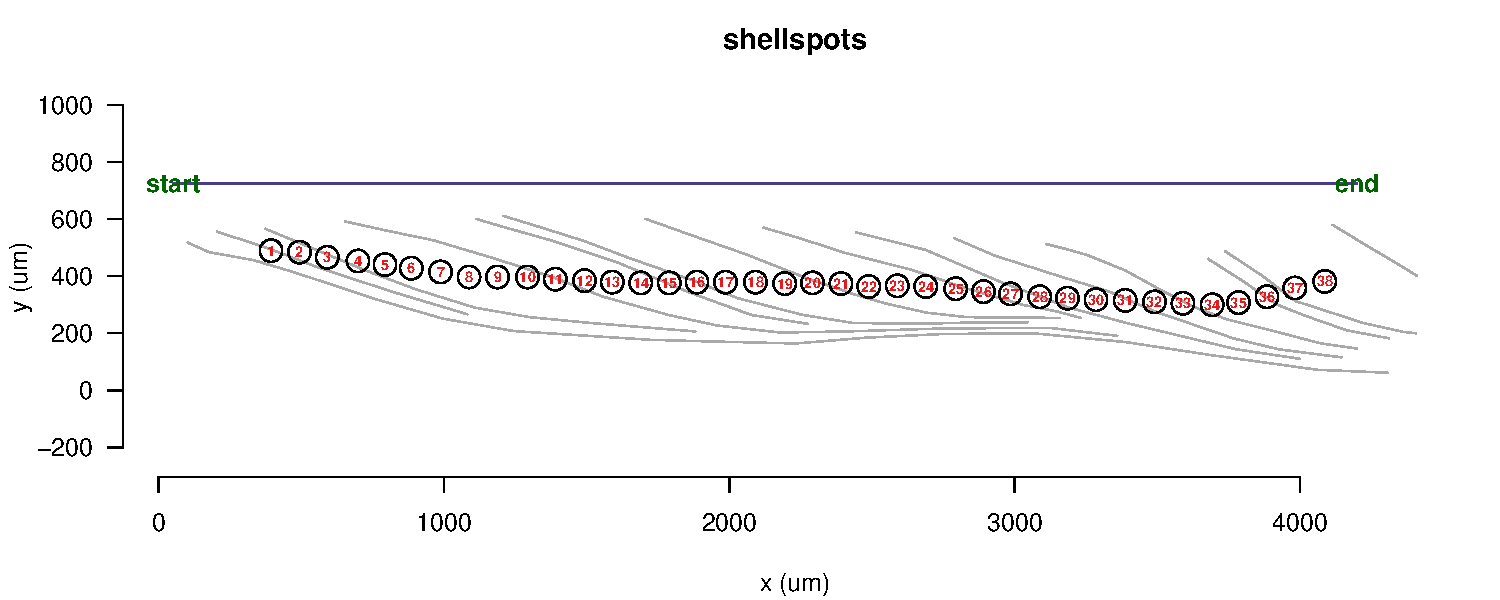
\includegraphics{sclero_tutorial-plot1}
\end{center}
\caption{The digitized representation of the shell section. Red numbers show the location of the sample spots. Grey lines represent the marked growth lines and the purple line the main axis to which the sample spots will be aligned. Y-axis coordinates are flipped due to a difference in the coordinate system between R and ImageJ (Java).}
\label{Fig:rawDist}
\end{figure}

\subsection{Aligning sample spots} \label{sec:spot.dist}

\mnote{spot.dist} An object of class \texttt{rawDist} can be readily processed using the \texttt{spot.dist} function. First, the function projects the beginning of each growth line to the measurement axis ($L_1$ and $L_2$ in Figure \ref{Fig:traverse}). Then, the sample spots are aligned along the main axis in relation to the adjacent growth lines on both sides of a sample spot such that $d_1/d_2 = d_{L_1}/d_{L_2}$.

\begin{figure}[h]
\begin{center}
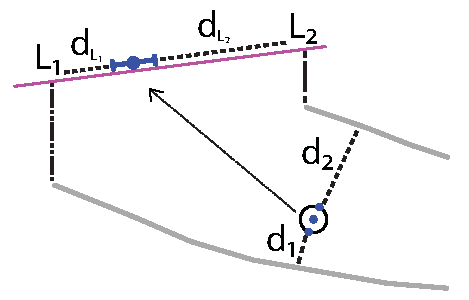
\includegraphics[width=0.5\textwidth]{spot_alignment.pdf}
\caption{Alignment of sample spots along the distance (main) axis. Grey lines represent ImageJ marked growth lines, open black circle a sample spot, and blue dots the centroid and the closest points to the adjacent growth lines along the perimeter of the sample spot. The \texttt{spot.dist} function aligns the blue dots such that $d_1/d_2 = d_{L_1}/d_{L_2}$ resulting to a segment along the distance axis (blue dot with error bars). Only the centroid is used, if sample spot areas are not specified separately (see Section \ref{sec:averaging_error}). The figure is from \citet{d18O_paper}}
\label{Fig:traverse}
\end{center}
\end{figure}

\mnote{plot.
spotDist} The function returns a list of class \texttt{spotDist} containing new information of the aligned sample spots and the digitized representation of the shell cross-section, which was already included in the \texttt{rawDist} object. Also \texttt{spotDist} objects can be plotted using the generic plotting command.

\begin{figure}[H]
\begin{center}
\begin{Schunk}
\begin{Sinput}
 aligned <- spot.dist(shell)
 plot(aligned)
\end{Sinput}
\end{Schunk}
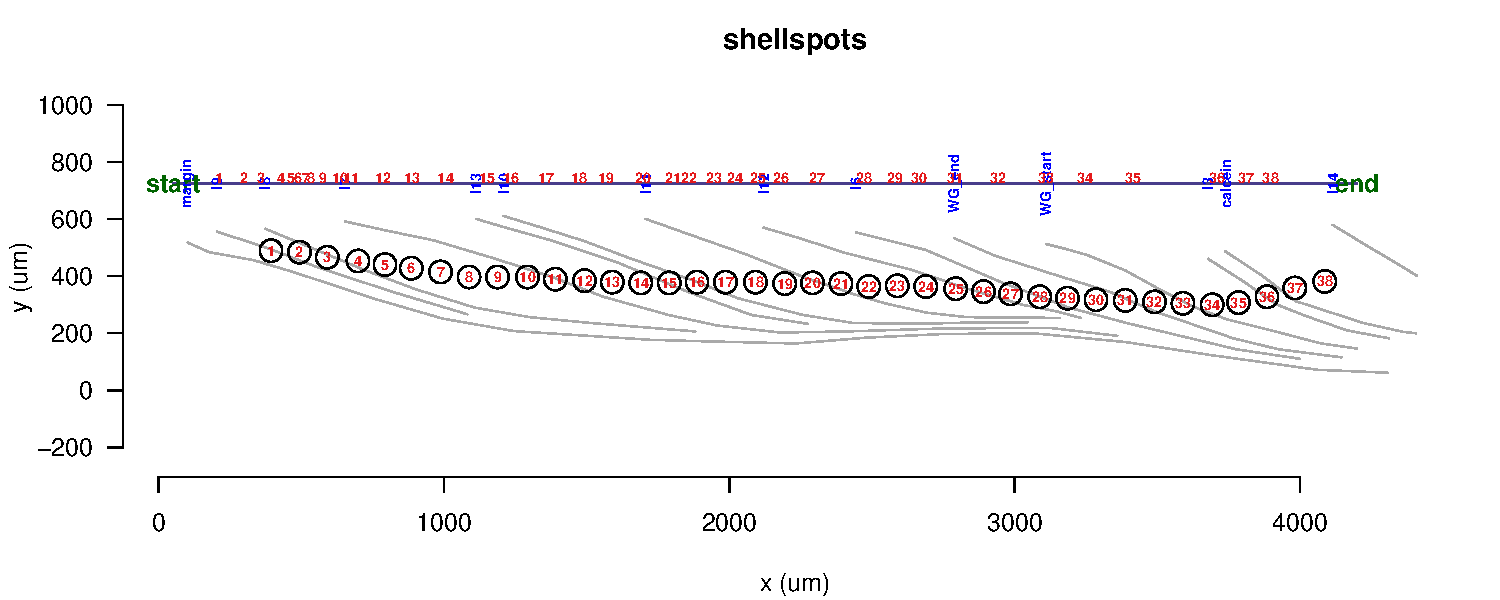
\includegraphics{sclero_tutorial-plot2}
\end{center}
\caption{Aligned sample spots along the measurement axis together with the digitized presentation from Figure \ref{Fig:rawDist}.}
\end{figure}

Typing the name of a \texttt{spotDist} object prints summarized information about the sample spot alignment:

\begin{Schunk}
\begin{Sinput}
 aligned
\end{Sinput}
\begin{Soutput}
"spotDist" object for shellspots
Main axis type: along
Scaling factor: 0.7812 pixels/um

Including following elements:
       list.elements       type ncol nrow length
 spots               list          0    0      1
 gbs                 psp           0    0      5
 main                psp           0    0      5
 window              owin          0    0      4
 start.main          ppp           0    0      6
 end.main            ppp           0    0      6
 sample.name         character     0    0      1
 scaling.factor      numeric       0    0      1
 unit                character     0    0      1
 main.type           character     0    0      1
 gb.projections      ppp           0    0      6
 gb.start            ppp           0    0      6
 gb.end              ppp           0    0      6
 gb.projections.dist data.frame    4   14      4
 mid.point.type      character     0    0      1
 det.dat             list          0    0      1
 output              list          0    0      1

Sample spot output:
 spot       dist
   1    94.62051
   2   182.55956
   3   243.07346
   4   311.18224
   5   346.60488
   6   372.90810
   7   399.64695
   8   417.83668
   9   458.90261
   10  505.31901
   11  544.43780
   12  656.68984
   13  758.02466
   14  874.91661
   15 1019.98703
   16 1105.41540
   17 1226.03512
   18 1341.27597
   19 1437.40469
   20 1567.85498
   21 1670.48644
   22 1729.37731
   23 1815.60525
   24 1889.99943
   25 1968.36939
   26 2048.81858
   27 2174.97867
   28 2341.48465
   29 2449.03098
   30 2534.59278
   31 2660.58426
   32 2811.12793
   33 2978.10571
   34 3115.26282
   35 3283.93206
   36 3577.47434
   37 3680.41824
   38 3765.36259

Growth line output:
     line             gap gap.l.main     dist0
 margin   margin-l9        102.40655    0.0000
 l9       l9-l8            168.97081  102.4066
 l8       l8-l7            279.05786  271.3774
 l7       l7-l13           459.54941  550.4352
 l13      l13-l10           96.00614 1009.9846
 l10      l10-l11          497.95187 1105.9908
 l11      l11-l12          413.46646 1603.9427
 l12      l12-l6           325.14081 2017.4091
 l6       l6-WG_end        343.06196 2342.5499
 WG_end   WG_end-WG_start  322.58065 2685.6119
 WG_start WG_start-l3      565.79621 3008.1925
 l3       l3-calcein        61.44393 3573.9887
 calcein  calcein-l14      375.06400 3635.4327
 l14      NA                      NA 4010.4967
\end{Soutput}
\end{Schunk}

The alignment information with sample spot numbers is stored as a sublist called \texttt{output} and can be extracted to a data.frame (see below). Otherwise the object behaves like any list in R. Relevant data can be subset as needed. Detailed data containing information of the alignment process is stored in a sublist called \texttt{det.dat}.

\begin{Schunk}
\begin{Sinput}
 aligned$output ## Results shown above
 aligned$det.dat ## Results not shown here to save space
\end{Sinput}
\end{Schunk}

\subsubsection{\texttt{spot.dist} settings} \label{sec:settings}

The alignment function \texttt{spot.dist} can either project growth lines on the distance (main) axis as in Figure \ref{Fig:traverse} or use the crossing points between growth lines and the main axis. These two types of the main axis can be used for different applications. The main axis type is automatically selected by the following criteria:

\begin{description}
  \item[along] Appropriate for samples with cut-off growth lines such as bivalve margin cross-sections and tree, sediment or ice-cores. This option is selected by placing the measurement axis such that \textbf{it does not cross any of the marked growth lines}. The location of each growth line is projected along the measurement axis from the beginning of the growth line (the point where you started marking the growth line in ImageJ).
  \item[cross] Appropriate for approximately round cross-sections: samples where the growth lines continue through the entire width of the sample (such as tree, coral or calcareous algae cross-sections and umbo-regions of bivalves). This type is selected by making the \textbf{main axis to cross each individual marked growth line}. The location of each growth line along the main axis is considered as a crossing point.
\end{description}

These criteria are set due to the need of defining a location for each marked growth line along the distance (main) axis. The choice is rigid, to simplify calculations, and to avoid bias in results by allowing two different methods for growth line locations. The easiest way to test which \texttt{type} suits a particular sample best is to save two sets of ImageJ zip files by moving the measurement axis.

\subsubsection{\texttt{spot.dist} troubleshooting}

Apart from the common issue of placing the main axis a wrong way around (because where you start drawing the line is considered as the \texttt{start} point), problems with \texttt{spot.dist} failing to find a location for each sample spot are often connected with the lack of marked growth lines on both sides of each sample spot. If this is the case, try drawing more growth lines so that each sample spot is surrounded by them. %If the nature of your sample material does not allow this, \texttt{spot.dist} function has an \texttt{alignment} option. Changing the value to \texttt{'traverse'} aligns the sample spots as described in Fig X and is sometimes helpful especially if you try to align samples along an entire cross-section of a curved material, such as a bivalve shell. However, changing the value will change the way your sample spots are aligned and should be done consistently. The \texttt{'closest'} option for \texttt{alignment} works best for applications described in this tutorial.

All functions in this package are still at an experimental stage. They do work for the applications needed by the author, but might not work for other applications. They are also likely to contain bugs, which can be fixed. Please contact the package maintainer, if you encounter unexpected behavior or obvious errors in the functions.

\clearpage
\subsection{Estimating spatial averaging error of sample spots} \label{sec:averaging_error}

The \sclero package can estimate the size of each sample spot, if size information is available. Size information can be assigned using the `Oval', `Elliptical', and `Rectangular selections' tools in ImageJ. To illustrate the process, we use the example above. 

\subsubsection{Add sample spot size information in ImageJ}

\begin{enumerate}
\item Open the shellspots.png and shellspots.zip files you saved in the previous steps. Both of these files are available in the \texttt{extdata} folder of the \sclero package. 
\item Select the `Oval selections' tool and mark the outline of the first sample spot. You can get circles by pressing down \textit{Shift} button while you do the marking. After releasing the mouse, you can still adjust the position of the circle. Once you are satisfied with the size and position of the circle, add the selection to ROI manager (\textit{Ctrl + T} or \textit{Cmd + T} depending on the OS).
\begin{figure}[H]
\begin{center}
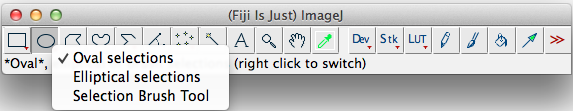
\includegraphics[width = 0.8\textwidth]{oval_selection.png}
\end{center}
\end{figure}
\item Then proceed to the next sample spot and mark it similarly. Mark all the sample spots within the shell section. Note that the order you mark the sample spots does not matter as the \sclero functions will associate centroid of each sample spot with individual sample spots in a sample spot sequence (\texttt{spots} in a \texttt{rawDist} object). The `Multi-point' tool marks, however, have to be inside each circle for the routine to work: the perimeters of spot size selections can cross each other, but the centroid of each selection has to be kept adjacent to a `Multi-point' tool mark.
\begin{figure}[H]
\begin{center}
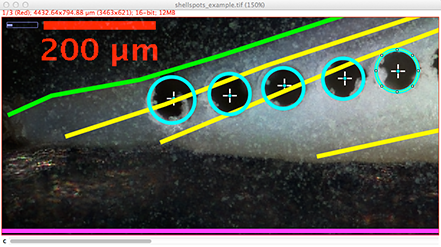
\includegraphics[width = 0.8\textwidth]{adding_ovals.png}
\end{center}
\end{figure}
\item Once you have marked all the sample spots using the `Oval selections' tool, save the content of the ROI manager as shellspots.zip. You can overwrite the old file (in fact, if you examine the shellspots.zip file included in the package, you will find out that it already contains spot size information).
\begin{figure}[H]
\begin{center}
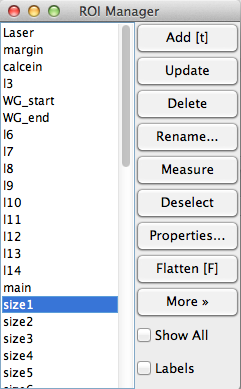
\includegraphics[width = 0.25\textwidth]{roi_manager_size.png}
\end{center}
\end{figure}
\end{enumerate}

\subsubsection{Calculating shell spot size and maximum extent along distance axis}

We can either re-read the shellspots.zip file into R (see Section \ref{sec:read.ijdata}) or use the \texttt{rawDist} object (\texttt{shell}), which has already been loaded to R. In here we assume that the user has followed the steps above and has \texttt{shell} object loaded in R. If not, run the following code:

\begin{Schunk}
\begin{Sinput}
 data(shellspots)
 shell <- convert.ijdata(shellspots)
\end{Sinput}
\end{Schunk}

\mnote{assign.
size} Assigning the sample spot sizes to \texttt{rawDist} objects is done using the \texttt{assign.size} function. If the .zip file containing spot size information is the same than from which the \texttt{rawDist} object was derived from and located in your working directory, assignment of spot sizes is simply specified by \texttt{assign.size(name\_of\_the\_rawDist\_object)}. This tutorial, however, uses the datasets included in the \sclero package and the path of the shellspots.zip file has to be specified.

\begin{Schunk}
\begin{Sinput}
 path <- file.path(system.file("extdata", package = "sclero"))
 shellsizes <- assign.size(shell, path = path)
\end{Sinput}
\end{Schunk}
\mnote{size
information} Sample spot area and diameter can now be extracted from the \texttt{rawDist} object.
\begin{Schunk}
\begin{Sinput}
 head(shellsizes$spot.area$spot.dat[[1]])
\end{Sinput}
\begin{Soutput}
Hyperframe:
  spot dist2spot spot.owin.name spot.owins spot.area spot.diameter
1    1  4.615401          size1     (owin)  5271.123      81.92446
2    2  3.263581 0001-0378-0383     (owin)  4479.683      75.52411
3    3  3.732048 0001-0365-0459     (owin)  4181.123      72.96397
4    4  1.280082 0001-0355-0546     (owin)  4329.116      74.24404
5    5  1.280082 0001-0343-0620     (owin)  4329.116      74.24404
6    6  1.280082 0001-0334-0693     (owin)  4035.704      71.68390
\end{Soutput}
\end{Schunk}

\mnote{dist2spot} The \texttt{dist2spot} column specifies the shortest distance between recalculated spot centroid location and the sample spot location assigned using the `Multi-point' tool. This distance is used to associate each sample spot circle with a sample spot. 

\mnote{spot.dist
extent} Calculating the maximum extent of each sample spot along the distance (main) axis (Figure \ref{Fig:traverse}) can now be conducted using the \texttt{spot.dist} function. Centroids of marked spots are automatically used to estimate the location of sample spots along the main axis, and the results therefore slightly differ from those obtained in Section \ref{sec:spot.dist}.

\begin{Schunk}
\begin{Sinput}
 spotsizes <- spot.dist(shellsizes)
 head(spotsizes$output[[1]])
\end{Sinput}
\begin{Soutput}
  spot      dist  dist.min dist.max spot.area spot.diameter
1    1  99.74392  21.82515 215.3387  5271.123      81.92446
2    2 180.81162  77.35968 273.1909  4479.683      75.52411
3    3 244.93171 129.08129 331.0464  4181.123      72.96397
4    4 313.45954 214.39049 383.7175  4329.116      74.24404
5    5 344.50215 280.20636 408.4641  4329.116      74.24404
6    6 373.51313 316.56173 430.3051  4035.704      71.68390
\end{Soutput}
\end{Schunk}

The \texttt{output} element of a \texttt{spotDist} object now contains not only distance information on sample spot centroids (\texttt{dist} column), but also information on the extent (\texttt{dist.min} and \texttt{dist.max}), as well as spot area and diameter. The actual size of sample spots can now be plotted after a specification.

\begin{figure}[H]
\begin{center}
\begin{Schunk}
\begin{Sinput}
 plot(spotsizes, spot.size = "actual")
\end{Sinput}
\end{Schunk}
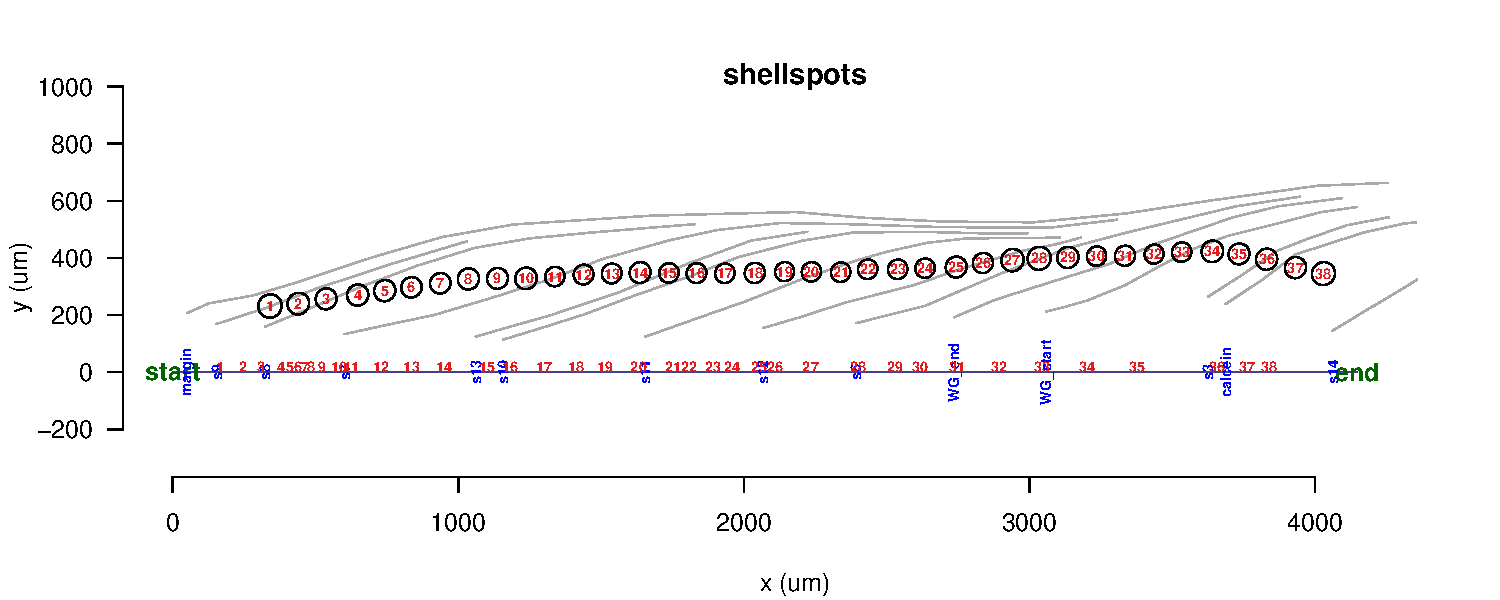
\includegraphics{sclero_tutorial-plotsize}
\end{center}
\caption{Aligned sample spots along the measurement axis together with the digitized presentation from Figure \ref{Fig:rawDist}. The circles represent the actual sizes of sample spots.}
\end{figure}

\clearpage
\subsection{Generating sample maps} \label{sec:maps}

Sometimes there is a need for plotting sampling results spatially in relation to sample spots. The \sclero package provides a function for such sample map plotting. As an example we use Ba/Ca ratios calculated from LA-ICP-MS measurements. The dataset is included in the package.

\begin{Schunk}
\begin{Sinput}
 data(barium)
 head(barium)
\end{Sinput}
\begin{Soutput}
  spots        Ba
1     1 1.3632722
2     2 1.2361042
3     3 1.1321925
4     4 1.0114307
5     5 0.8961586
6     6 0.7422160
\end{Soutput}
\end{Schunk}

We load the \texttt{rawDist} object \texttt{shellsizes} from the example in Section \ref{sec:averaging_error}

\begin{Schunk}
\begin{Sinput}
 data(shellsizes)
\end{Sinput}
\end{Schunk}

\mnote{assign.
value} The assignment of values is conducted using the \texttt{assign.value} function, where \texttt{value} is a data frame with a value for each sample spot. NA's are allowed values and lead to white sample spots. The \texttt{spot.type} argument has to be \texttt{"value"} or \texttt{"idvalue"} for density plotting.

\begin{figure}[H]
\begin{center}
\begin{Schunk}
\begin{Sinput}
 shellvalues <- assign.value(shellsizes, barium, value.name = "Ba/Ca")
 plot(shellvalues, spot.size = "actual", spot.type = "value", main.type = "none")
\end{Sinput}
\end{Schunk}
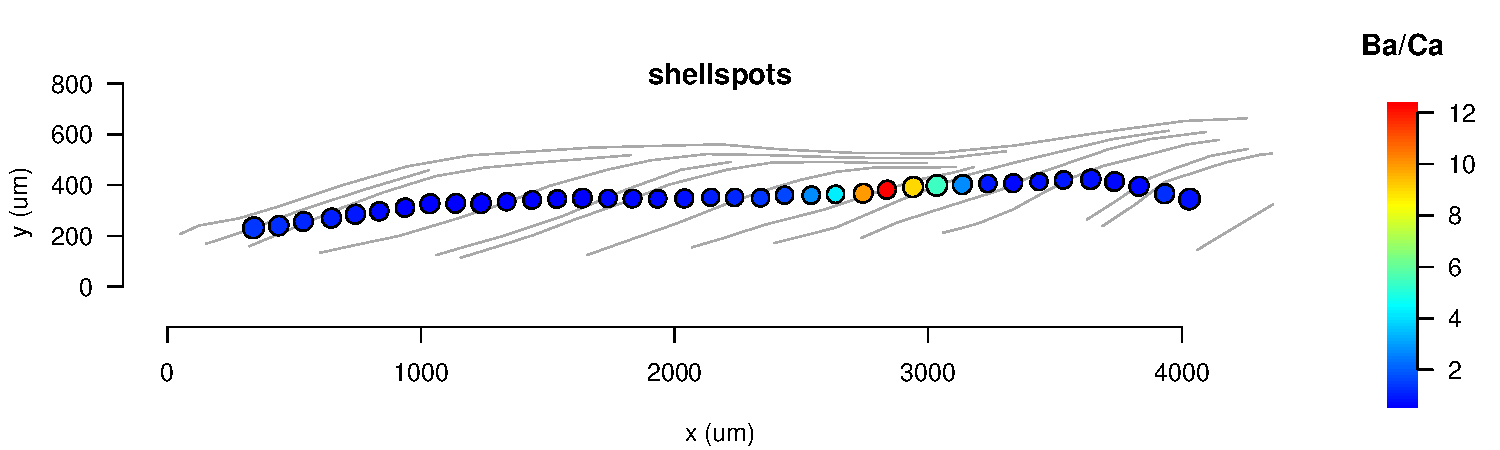
\includegraphics{sclero_tutorial-plotvalues}
\end{center}
\caption{Spatial density map of Ba/Ca over the shell sequence. The \texttt{spot.type} argument has to be \texttt{"value"} or \texttt{"idvalue"} to generate such maps. The \texttt{main.type} argument is used to remove the distance axis.}
\end{figure}

A \texttt{rawDist} object with value information can be run through the \texttt{spot.dist} function and plotted like any \texttt{spotDist} object

\begin{figure}[H]
\begin{center}
\begin{Schunk}
\begin{Sinput}
 shellvalues.aligned <- spot.dist(shellvalues)
 plot(shellvalues.aligned, spot.size = "actual", spot.type = "idvalue",
   spot.color = "darkgrey", highlight.gbs = c("WG_start", "WG_end"))
\end{Sinput}
\end{Schunk}
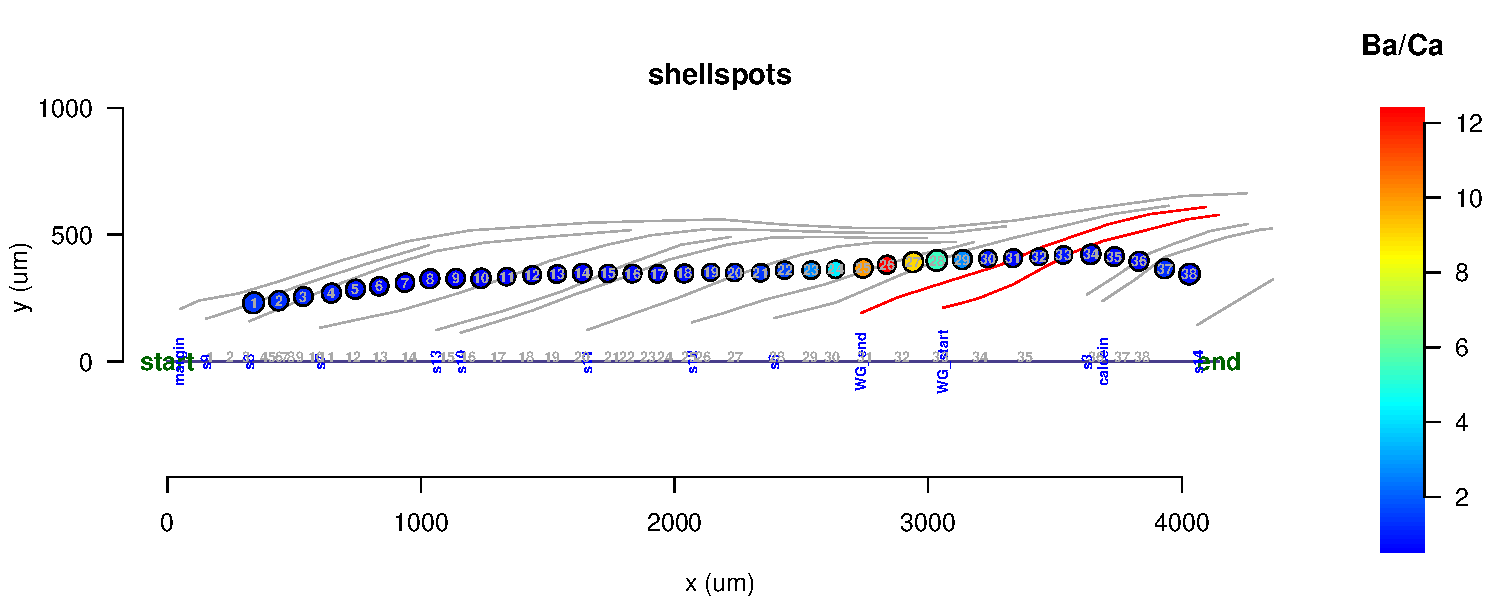
\includegraphics{sclero_tutorial-plotvaluesalign}
\end{center}
\caption{Spatial density map using a \texttt{spotDist} object. The beginning and the end of a winter growth band (\textit{"WG\_start"} and \textit{"WG\_end"}) are highlighted and sample spot sequence color specified using the \texttt{spot.color} argument.
}
\end{figure}

\clearpage
\subsection{Aligning multiple sample spot sequences} \label{sec:multiple}

Multiple spot sequences can be aligned with the \sclero package similarly to single spot sequences. These spot sequences must be specified using separate `Multi-point' tool ROI objects for each sequence. In the following example included to the package we use an ImageJ .zip file with a LA-ICP-MS (Laser) sequence and three secondary ion micro-probe (SIMS) sequences. All of the sequences are specified as separate ROIs.

\begin{figure}[H]
\begin{center}
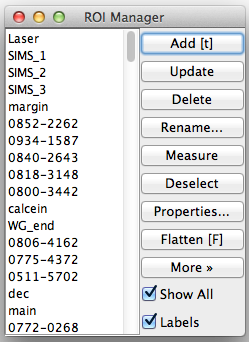
\includegraphics[width = 0.25\textwidth]{roi_manager_multi.png}
\end{center}
\end{figure}

The alignment procedure is similar to single sequences (see Sections \ref{sec:read.ijdata} and \ref{sec:spot.dist}) with the exception that it now produces alignment for each sequence separately.

\begin{Schunk}
\begin{Sinput}
 file <- file.path(system.file("extdata", package = "sclero"), "multi_spotseq.zip")
 dat <- read.ijdata(file, scale = 0.7812, unit = "um")
 multispot.raw <- convert.ijdata(dat)
 path <- file.path(system.file("extdata", package = "sclero"))
 multispot.size <- assign.size(multispot.raw, path = path)
 multispot <- spot.dist(multispot.size)
\end{Sinput}
\end{Schunk}

\begin{figure}[H]
\begin{center}
\begin{Schunk}
\begin{Sinput}
 plot(multispot, spot.size = "actual")
\end{Sinput}
\end{Schunk}
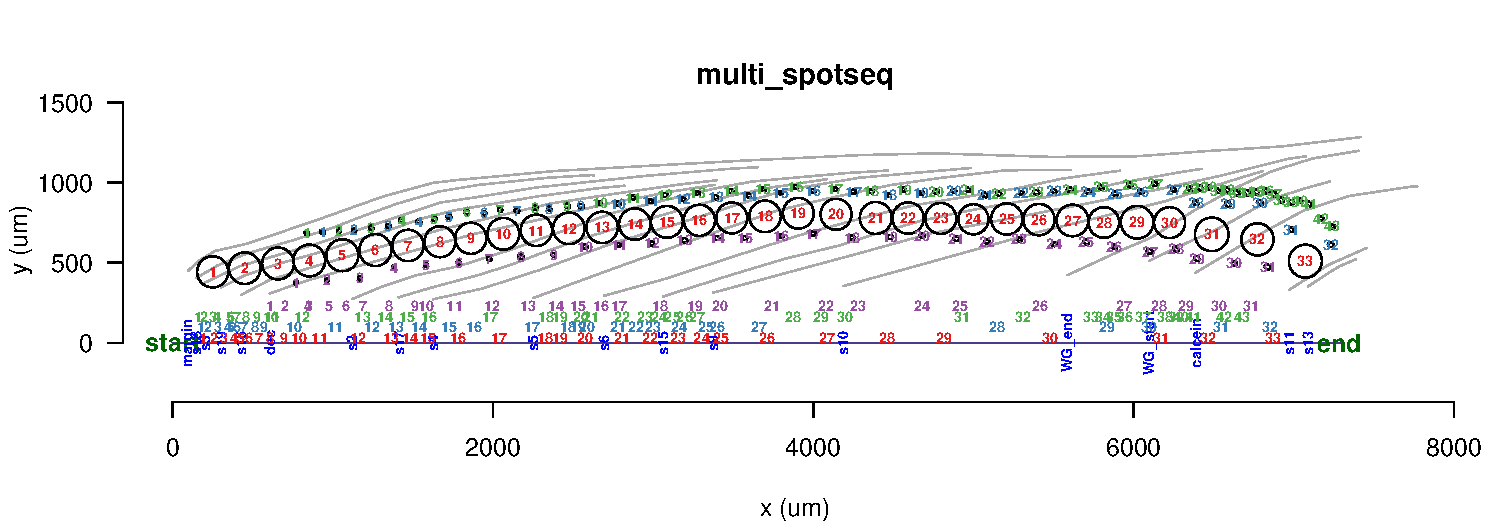
\includegraphics{sclero_tutorial-multispot}
\end{center}
\caption{A sample spot sequences with multiple sequences become aligned independently of each other.}
\end{figure}

\section{Graphics used in the \sclero package}

The \sclero package currently uses the \textit{graphics} package distributed with R for plotting. Plotting sample maps is carried out by the \texttt{sclero:::samplemap} function, which works as an internal function and therefore has not been exported. Users willing to modify \sclero plots beyond the flexibility allowed by \texttt{plot.rawDist} and \texttt{plot.spotDist} functions are instructed to modify the \texttt{samplemap} function, which consists of standard R graphics syntax. It should be noted that \texttt{sclero:::samplemap} function calls for the \href{https://stat.ethz.ch/R-manual/R-devel/library/graphics/html/layout.html}{\texttt{layout}} function every time the arguments \texttt{spot.type = "value"} or \texttt{spot.type = "idvalue"} are used. Consequently, the graphics window is divided into two regions that might cause issues when combining \sclero plots with other graphics. The users are adviced to consider the graphics window resetting procedure specified in \href{https://stat.ethz.ch/R-manual/R-devel/library/graphics/html/layout.html}{\texttt{layout}} examples. Any user willing to create a more flexible plotting functionality for \sclero are asked to contact the package maintainer.

\section{Dependencies}

The sclero package depends on:

\begin{description}
\item[RImageJROI] \citep{RImageJROI}. Used to import ImageJ ROI objects to R.
\item[spatstat] \citep{Baddeley2005}. Used for geometric calculations.
\item[plyr] \citep{Wickham2011}. Used for quicker and easier list calculations. 
\end{description}

\bibliographystyle{abbrvnat}
\bibliography{bibliography}

\end{document}
